\documentclass[leqno]{article}
\usepackage[utf8]{inputenc}
\usepackage{enumitem}
\usepackage{tikz}
\usepackage[parfill]{parskip}
\usepackage{mathtools}
\usepackage{amsmath}
\usepackage{amssymb}

\title{Computationele logica}
\author{
    Kamans, Jim\\
    \texttt{10302905}
    \and
    Roosingh, Sander\\
    \texttt{11983957}
    \and
    Schenk, Stefan\\
    \texttt{11881798}
}
\date{December 2017}

\begin{document}

\maketitle

%%%%%%%%%%%%%%%%%%%%%%%%%%%%%%%%%%%%%%%%%%%%%%%%%%%%%%%%%%%%%%%%%%%%%%%%%%%%%%%
%% Exercise 1 %%
%%%%%%%%%%%%%%%%%%%%%%%%%%%%%%%%%%%%%%%%%%%%%%%%%%%%%%%%%%%%%%%%%%%%%%%%%%%%%%%
\section*{Exercise 1}
A robot is in a war zone. It doesn’t know its location, but all it cares is
whether or not there is a mine in front (m), and whether or not there is an
enemy approaching (e).

\begin{enumerate}
  \item \textit{Represent the robot's belief-revision structure using a single-agent plausibility model.}

  \begin{center}
  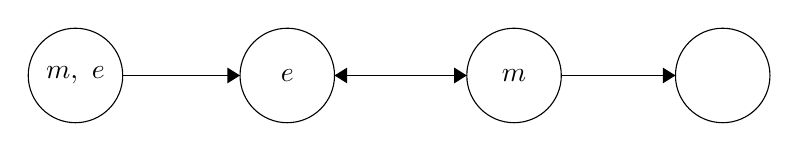
\begin{tikzpicture}[scale=0.2]
  \tikzstyle{every node}+=[inner sep=0pt]
  \draw [black] (35.95,-14.6) circle (3);
  \draw (35.95,-14.6) node {$e$};
  \draw [black] (50.35,-14.6) circle (3);
  \draw (50.35,-14.6) node {$m$};
  \draw [black] (63.6,-14.6) circle (3);
  \draw [black] (22.5,-14.6) circle (3);
  \draw (22.5,-14.6) node {$m,\mbox{ }e$};
  \draw [black] (38.95,-14.6) -- (47.35,-14.6);
  \fill [black] (47.35,-14.6) -- (46.55,-14.1) -- (46.55,-15.1);
  \draw [black] (47.35,-14.6) -- (38.95,-14.6);
  \fill [black] (38.95,-14.6) -- (39.75,-15.1) -- (39.75,-14.1);
  \draw [black] (25.5,-14.6) -- (32.95,-14.6);
  \fill [black] (32.95,-14.6) -- (32.15,-14.1) -- (32.15,-15.1);
  \draw [black] (53.35,-14.6) -- (60.6,-14.6);
  \fill [black] (60.6,-14.6) -- (59.8,-14.1) -- (59.8,-15.1);
  \end{tikzpicture}
  \end{center}

  \item \textit{Suppose now that the robot’s sensors indicate some vibrations.}

  \begin{center}
  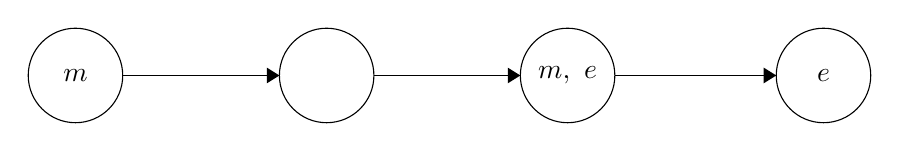
\begin{tikzpicture}[scale=0.2]
  \tikzstyle{every node}+=[inner sep=0pt]
  \draw [black] (65.45,-11.7) circle (3);
  \draw (65.45,-11.7) node {$e$};
  \draw [black] (17.95,-11.7) circle (3);
  \draw (17.95,-11.7) node {$m$};
  \draw [black] (33.9,-11.7) circle (3);
  \draw [black] (49.2,-11.7) circle (3);
  \draw (49.2,-11.7) node {$m,\mbox{ }e$};
  \draw [black] (20.95,-11.7) -- (30.9,-11.7);
  \fill [black] (30.9,-11.7) -- (30.1,-11.2) -- (30.1,-12.2);
  \draw [black] (36.9,-11.7) -- (46.2,-11.7);
  \fill [black] (46.2,-11.7) -- (45.4,-11.2) -- (45.4,-12.2);
  \draw [black] (52.2,-11.7) -- (62.45,-11.7);
  \fill [black] (62.45,-11.7) -- (61.65,-11.2) -- (61.65,-12.2);
  \end{tikzpicture}
  \end{center}

  \item \textit{Immediately after the event in the previous part, the robot’s metal detector indicates the presence of a mine.}

  \begin{center}
  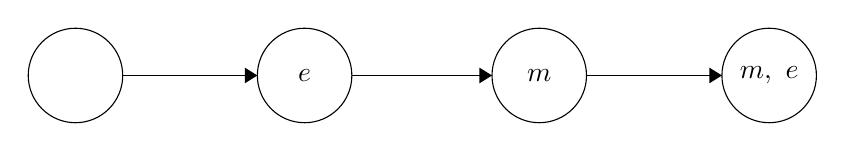
\begin{tikzpicture}[scale=0.2]
  \tikzstyle{every node}+=[inner sep=0pt]
  \draw [black] (35.95,-22.9) circle (3);
  \draw (35.95,-22.9) node {$e$};
  \draw [black] (50.85,-22.9) circle (3);
  \draw (50.85,-22.9) node {$m$};
  \draw [black] (21.4,-22.9) circle (3);
  \draw [black] (65.45,-22.9) circle (3);
  \draw (65.45,-22.9) node {$m,\mbox{ }e$};
  \draw [black] (24.4,-22.9) -- (32.95,-22.9);
  \fill [black] (32.95,-22.9) -- (32.15,-22.4) -- (32.15,-23.4);
  \draw [black] (38.95,-22.9) -- (47.85,-22.9);
  \fill [black] (47.85,-22.9) -- (47.05,-22.4) -- (47.05,-23.4);
  \draw [black] (53.85,-22.9) -- (62.45,-22.9);
  \fill [black] (62.45,-22.9) -- (61.65,-22.4) -- (61.65,-23.4);
  \end{tikzpicture}
  \end{center}

  \item \textit{Immediately after the previous two events, the robot receives a
  message from its controller, saying that: “(Right now, your vibration
  detector malfunctions, so)} \textbf{Whatever you currently believe about the
  enemy (approaching or not) is false.”}

  $\varphi \coloneqq Be \rightarrow \neg e \wedge B\neg e \rightarrow e$

  This is true in states: 1 and 3.

  \item \textit{Assume that the controller is known to be infallible, and so
  that the robot performs an update with the announced sentence. Represent the
  robots’s new belief structure (as a plausibility model) after this update.
  What does the robot believe about e and m after the update?}

  \begin{center}
  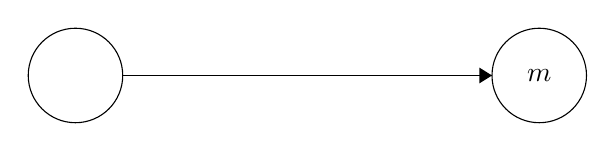
\begin{tikzpicture}[scale=0.2]
  \tikzstyle{every node}+=[inner sep=0pt]
  \draw [black] (50.85,-22.9) circle (3);
  \draw (50.85,-22.9) node {$m$};
  \draw [black] (21.4,-22.9) circle (3);
  \draw [black] (24.4,-22.9) -- (47.85,-22.9);
  \fill [black] (47.85,-22.9) -- (47.05,-22.4) -- (47.05,-23.4);
  \end{tikzpicture}
  \end{center}

  \item \textit{What would have been the final belief structure (plausibility
  model) of the robot if the above three events happened in a different order,
  namely: first the robot received the above message from the (infallible)
  controller, then its (strongly trusted) sensor indicated vibrations (hence
  enemies), and then its (strongly trusted) metal detector indicated a mine?}

  After the infallible controller message, and after the sensor indicated
  vibrations:
  \begin{center}
  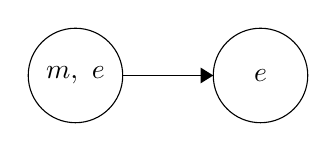
\begin{tikzpicture}[scale=0.2]
  \tikzstyle{every node}+=[inner sep=0pt]
  \draw [black] (39.15,-22.9) circle (3);
  \draw (39.15,-22.9) node {$e$};
  \draw [black] (27.4,-22.9) circle (3);
  \draw (27.4,-22.9) node {$m,\mbox{ }e$};
  \draw [black] (30.4,-22.9) -- (36.15,-22.9);
  \fill [black] (36.15,-22.9) -- (35.35,-22.4) -- (35.35,-23.4);
  \end{tikzpicture}
  \end{center}

  After the mine presence was detected:
  \begin{center}
  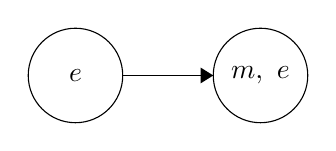
\begin{tikzpicture}[scale=0.2]
  \tikzstyle{every node}+=[inner sep=0pt]
  \draw [black] (39.15,-22.9) circle (3);
  \draw (39.15,-22.9) node {$m,\mbox{ }e$};
  \draw [black] (27.4,-22.9) circle (3);
  \draw (27.4,-22.9) node {$e$};
  \draw [black] (30.4,-22.9) -- (36.15,-22.9);
  \fill [black] (36.15,-22.9) -- (35.35,-22.4) -- (35.35,-23.4);
  \end{tikzpicture}
  \end{center}

\end{enumerate}

%%%%%%%%%%%%%%%%%%%%%%%%%%%%%%%%%%%%%%%%%%%%%%%%%%%%%%%%%%%%%%%%%%%%%%%%%%%%%%%
%% Exercise 2 %%
%%%%%%%%%%%%%%%%%%%%%%%%%%%%%%%%%%%%%%%%%%%%%%%%%%%%%%%%%%%%%%%%%%%%%%%%%%%%%%%
\section*{Exercise 2}
A covered coin is on the table, lying either Heads up (H) or Tails up (T).
There are two agents, Alice and Bob, and it is common knowledge that neither of
them can see the coin, but that for some reason they both believe that the coin
lies Tails up.

\begin{enumerate}

  \item \textit{Draw a multi-agent plausibility model M0 (with two agents, a
  for Alice and b for Bob, and atomic sentence H and T) to accurately represent
  all the information above.}

  \begin{center}
  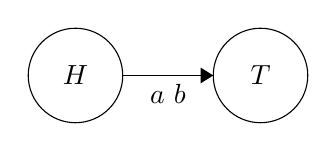
\begin{tikzpicture}[scale=0.2]
  \tikzstyle{every node}+=[inner sep=0pt]
  \draw [black] (39.15,-22.9) circle (3);
  \draw (39.15,-22.9) node {$T$};
  \draw [black] (27.4,-22.9) circle (3);
  \draw (27.4,-22.9) node {$H$};
  \draw [black] (30.4,-22.9) -- (36.15,-22.9);
  \fill [black] (36.15,-22.9) -- (35.35,-22.4) -- (35.35,-23.4);
  \draw (33.27,-23.4) node [below] {$a\mbox{ }b$};
  \end{tikzpicture}
  \end{center}

  \item \textit{Some external referee publicly announces: “The coin lies Heads
  up”. It is common knowledge that: Bob strongly trusts the referee, but that
  Alice is neutral towards the referee (neither trusts nor distrusts him).}

  \begin{center}
  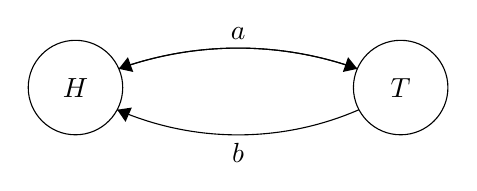
\begin{tikzpicture}[scale=0.2]
  \tikzstyle{every node}+=[inner sep=0pt]
  \draw [black] (48.05,-22.9) circle (3);
  \draw (48.05,-22.9) node {$T$};
  \draw [black] (27.4,-22.9) circle (3);
  \draw (27.4,-22.9) node {$H$};
  \draw [black] (30.15,-21.706) arc (109.64756:70.35244:22.529);
  \fill [black] (45.3,-21.71) -- (44.71,-20.97) -- (44.38,-21.91);
  \draw (37.73,-19.89) node [above] {$a$};
  \draw [black] (45.404,-24.307) arc (-66.47258:-113.52742:19.236);
  \fill [black] (30.05,-24.31) -- (30.58,-25.08) -- (30.98,-24.17);
  \draw (37.73,-26.41) node [below] {$b$};
  \draw [black] (30.15,-21.706) arc (109.65444:70.34556:22.522);
  \fill [black] (30.15,-21.71) -- (31.07,-21.91) -- (30.73,-20.97);
  \end{tikzpicture}
  \end{center}

  \item \textit{Represent (draw) a model for the situation after the action
  described in the previous part.}

  \begin{center}
  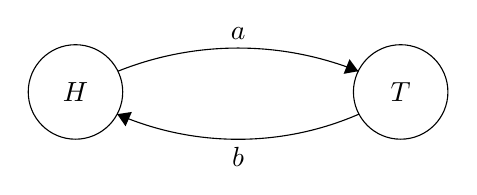
\begin{tikzpicture}[scale=0.2]
  \tikzstyle{every node}+=[inner sep=0pt]
  \draw [black] (48.05,-22.9) circle (3);
  \draw (48.05,-22.9) node {$T$};
  \draw [black] (27.4,-22.9) circle (3);
  \draw (27.4,-22.9) node {$H$};
  \draw [black] (45.404,-24.307) arc (-66.47258:-113.52742:19.236);
  \fill [black] (30.05,-24.31) -- (30.58,-25.08) -- (30.98,-24.17);
  \draw (37.73,-26.41) node [below] {$b$};
  \draw [black] (30.093,-21.584) arc (111.84686:68.15314:20.509);
  \fill [black] (45.36,-21.58) -- (44.8,-20.82) -- (44.43,-21.75);
  \draw (37.73,-19.61) node [above] {$a$};
  \end{tikzpicture}
  \end{center}

  \item \textit{Represent this action as an event plausibility model.}

  \begin{center}
  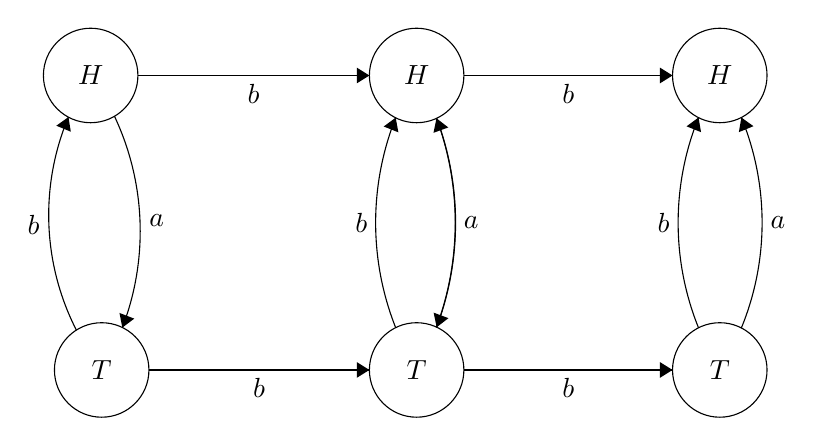
\begin{tikzpicture}[scale=0.2]
  \tikzstyle{every node}+=[inner sep=0pt]
  \draw [black] (23.7,-41.6) circle (3);
  \draw (23.7,-41.6) node {$T$};
  \draw [black] (23,-22.9) circle (3);
  \draw (23,-22.9) node {$H$};
  \draw [black] (43.7,-22.9) circle (3);
  \draw (43.7,-22.9) node {$H$};
  \draw [black] (43.7,-41.6) circle (3);
  \draw (43.7,-41.6) node {$T$};
  \draw [black] (62.95,-22.9) circle (3);
  \draw (62.95,-22.9) node {$H$};
  \draw [black] (62.95,-41.6) circle (3);
  \draw (62.95,-41.6) node {$T$};
  \draw [black] (22.094,-39.071) arc (-152.93628:-202.77619:16.066);
  \fill [black] (21.59,-25.54) -- (20.82,-26.09) -- (21.74,-26.47);
  \draw (19.79,-32.37) node [left] {$b$};
  \draw [black] (24.511,-25.487) arc (25.25619:-20.96867:17.105);
  \fill [black] (25.01,-38.91) -- (25.77,-38.34) -- (24.83,-37.98);
  \draw (26.69,-32.13) node [right] {$a$};
  \draw [black] (44.97,-25.614) arc (20.53371:-20.53371:18.918);
  \fill [black] (44.97,-38.89) -- (45.72,-38.31) -- (44.78,-37.96);
  \draw (46.67,-32.25) node [right] {$a$};
  \draw [black] (42.369,-38.915) arc (-158.37663:-201.62337:18.088);
  \fill [black] (42.37,-25.58) -- (41.61,-26.14) -- (42.54,-26.51);
  \draw (40.6,-32.25) node [left] {$b$};
  \draw [black] (44.96,-25.619) arc (20.35187:-20.35187:19.066);
  \fill [black] (44.96,-25.62) -- (44.77,-26.54) -- (45.71,-26.2);
  \draw [black] (64.319,-25.565) arc (22.31192:-22.31192:17.608);
  \fill [black] (64.32,-25.57) -- (64.16,-26.5) -- (65.09,-26.12);
  \draw (66.14,-32.25) node [right] {$a$};
  \draw [black] (61.6,-38.925) arc (-158.02958:-201.97042:17.842);
  \fill [black] (61.6,-25.57) -- (60.84,-26.13) -- (61.76,-26.5);
  \draw (59.8,-32.25) node [left] {$b$};
  \draw [black] (46.7,-41.6) -- (59.95,-41.6);
  \fill [black] (59.95,-41.6) -- (59.15,-41.1) -- (59.15,-42.1);
  \draw (53.33,-42.1) node [below] {$b$};
  \draw [black] (46.7,-22.9) -- (59.95,-22.9);
  \fill [black] (59.95,-22.9) -- (59.15,-22.4) -- (59.15,-23.4);
  \draw (53.33,-23.4) node [below] {$b$};
  \draw [black] (26,-22.9) -- (40.7,-22.9);
  \fill [black] (40.7,-22.9) -- (39.9,-22.4) -- (39.9,-23.4);
  \draw (33.35,-23.4) node [below] {$b$};
  \draw [black] (26.7,-41.6) -- (40.7,-41.6);
  \fill [black] (40.7,-41.6) -- (39.9,-41.1) -- (39.9,-42.1);
  \draw (33.7,-42.1) node [below] {$b$};
  \end{tikzpicture}
  \end{center}

  \item \textit{Starting from the original situation (in part 1), suppose the
  action that we described in the previous part happens.}

  \begin{center}
  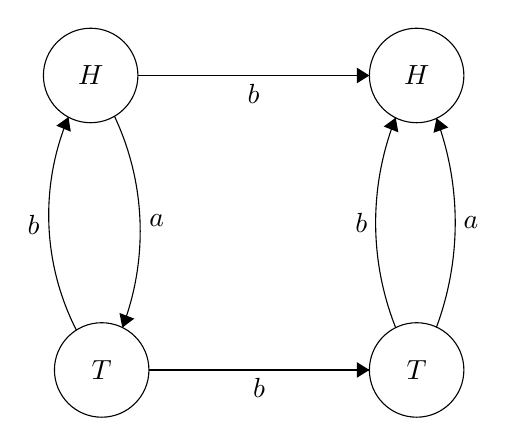
\begin{tikzpicture}[scale=0.2]
  \tikzstyle{every node}+=[inner sep=0pt]
  \draw [black] (23.7,-41.6) circle (3);
  \draw (23.7,-41.6) node {$T$};
  \draw [black] (23,-22.9) circle (3);
  \draw (23,-22.9) node {$H$};
  \draw [black] (43.7,-22.9) circle (3);
  \draw (43.7,-22.9) node {$H$};
  \draw [black] (43.7,-41.6) circle (3);
  \draw (43.7,-41.6) node {$T$};
  \draw [black] (22.094,-39.071) arc (-152.93628:-202.77619:16.066);
  \fill [black] (21.59,-25.54) -- (20.82,-26.09) -- (21.74,-26.47);
  \draw (19.79,-32.37) node [left] {$b$};
  \draw [black] (24.511,-25.487) arc (25.25619:-20.96867:17.105);
  \fill [black] (25.01,-38.91) -- (25.77,-38.34) -- (24.83,-37.98);
  \draw (26.69,-32.13) node [right] {$a$};
  \draw [black] (42.369,-38.915) arc (-158.37663:-201.62337:18.088);
  \fill [black] (42.37,-25.58) -- (41.61,-26.14) -- (42.54,-26.51);
  \draw (40.6,-32.25) node [left] {$b$};
  \draw [black] (44.96,-25.619) arc (20.35187:-20.35187:19.066);
  \fill [black] (44.96,-25.62) -- (44.77,-26.54) -- (45.71,-26.2);
  \draw (46.65,-32.25) node [right] {$a$};
  \draw [black] (26,-22.9) -- (40.7,-22.9);
  \fill [black] (40.7,-22.9) -- (39.9,-22.4) -- (39.9,-23.4);
  \draw (33.35,-23.4) node [below] {$b$};
  \draw [black] (26.7,-41.6) -- (40.7,-41.6);
  \fill [black] (40.7,-41.6) -- (39.9,-41.1) -- (39.9,-42.1);
  \draw (33.7,-42.1) node [below] {$b$};
  \end{tikzpicture}
  \end{center}

\end{enumerate}

\end{document}
